\documentclass[a4paper, 12pt]{article}
\usepackage{graphicx}
\usepackage{listings}

\setlength\parindent{24pt}

\lstset{language=c++,breaklines=true, frame=single}

\begin{document}

\begin{figure}
    \centering
    
\includegraphics[width=1\textwidth]{Logo}
\end{figure}

\title{Assignment Report}
\author{Manwel Bugeja}
\date{\today}
\maketitle

\tableofcontents
\newpage

\section{Introduction}
This assignment is implemented in c++. 

\section{Question 1}
\subsection{How the problem was tackled} 
First off, an FSA was dedigned to accept numbers. Then the required structures where initialized in code.
The FSA was translated to code in the form of transition table. Then, code was developed to successfully read the 
numbers with a stack and rollback capabilities. This was done according to the pseudo code provided in the text book.
Following that, more and more elements where added, testing the lexer as it grew.

\subsection{Data Structures}
The following structures are defined in "transitions.h".
Three enumerations were done to keep track of classifiers, states and token types. The enum for token types is divided
into two parts (shown via the comment). The second part is used exclusivly by the parser.

An array of accepting states was declared to keep track of the states which were final.
The transisition table was implemented as a 2d array with classifiers as columns and states as rows.

The char\_cat and type tables were implemented as functions.

\subsection{FSA}

The following are parts of the FSA in the order they where added to the transition table.

\begin{figure}[h]
    \centering
    \frame{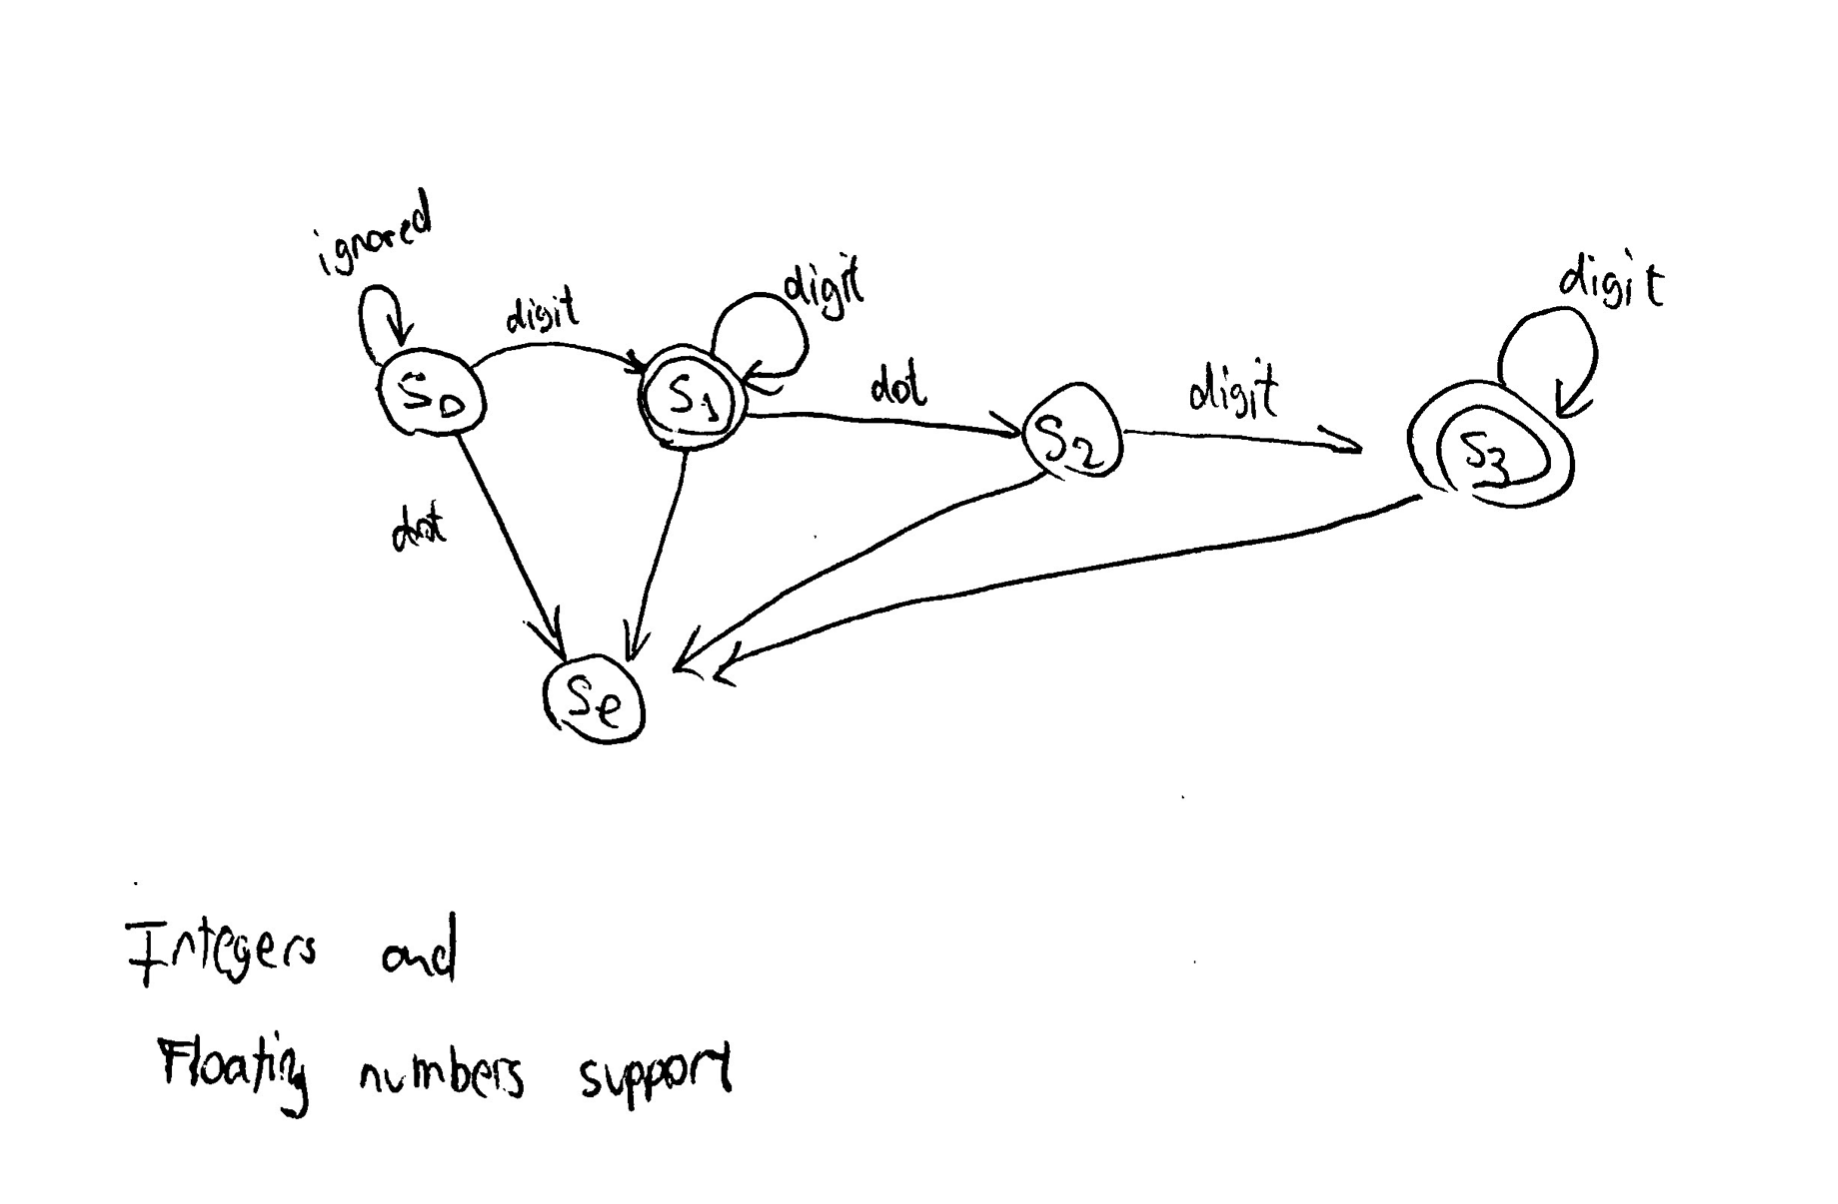
\includegraphics[width=1\textwidth]{images/numbers}}
    \caption{FSA (part concerned with numbers)}
\end{figure}

\begin{figure}[h]
    \centering
    \frame{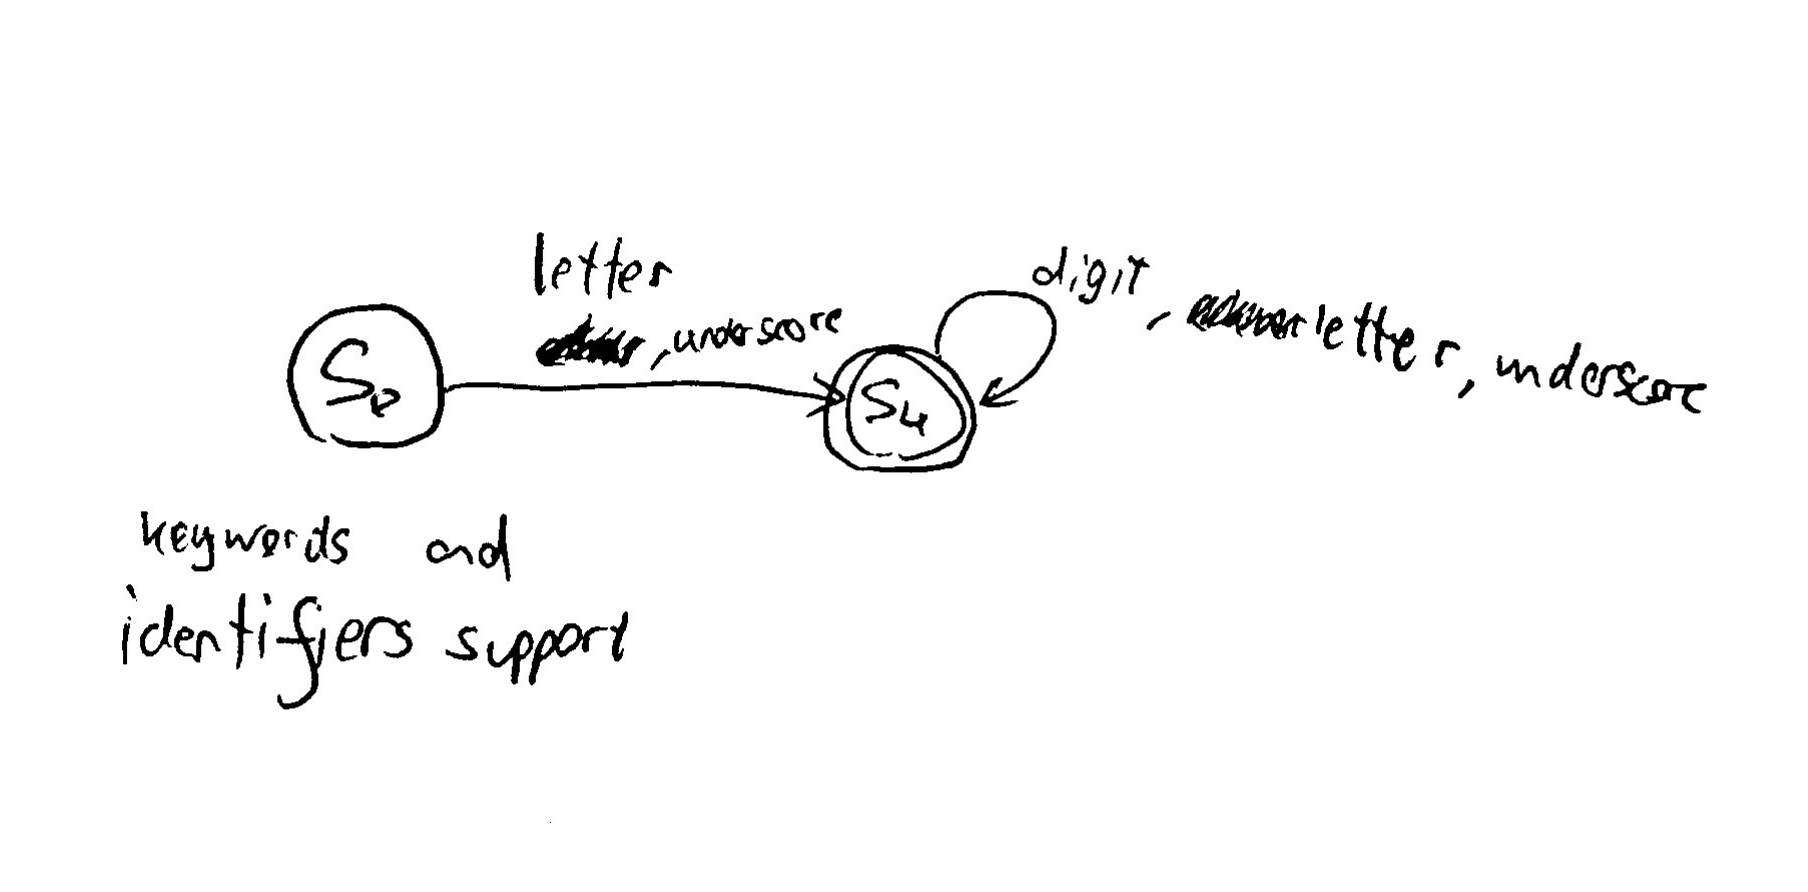
\includegraphics[width=1\textwidth]{images/identifiers}}
    \caption{FSA (part concerned with identifiers and keywords)}
\end{figure}

\begin{figure}[h]
    \centering
    \frame{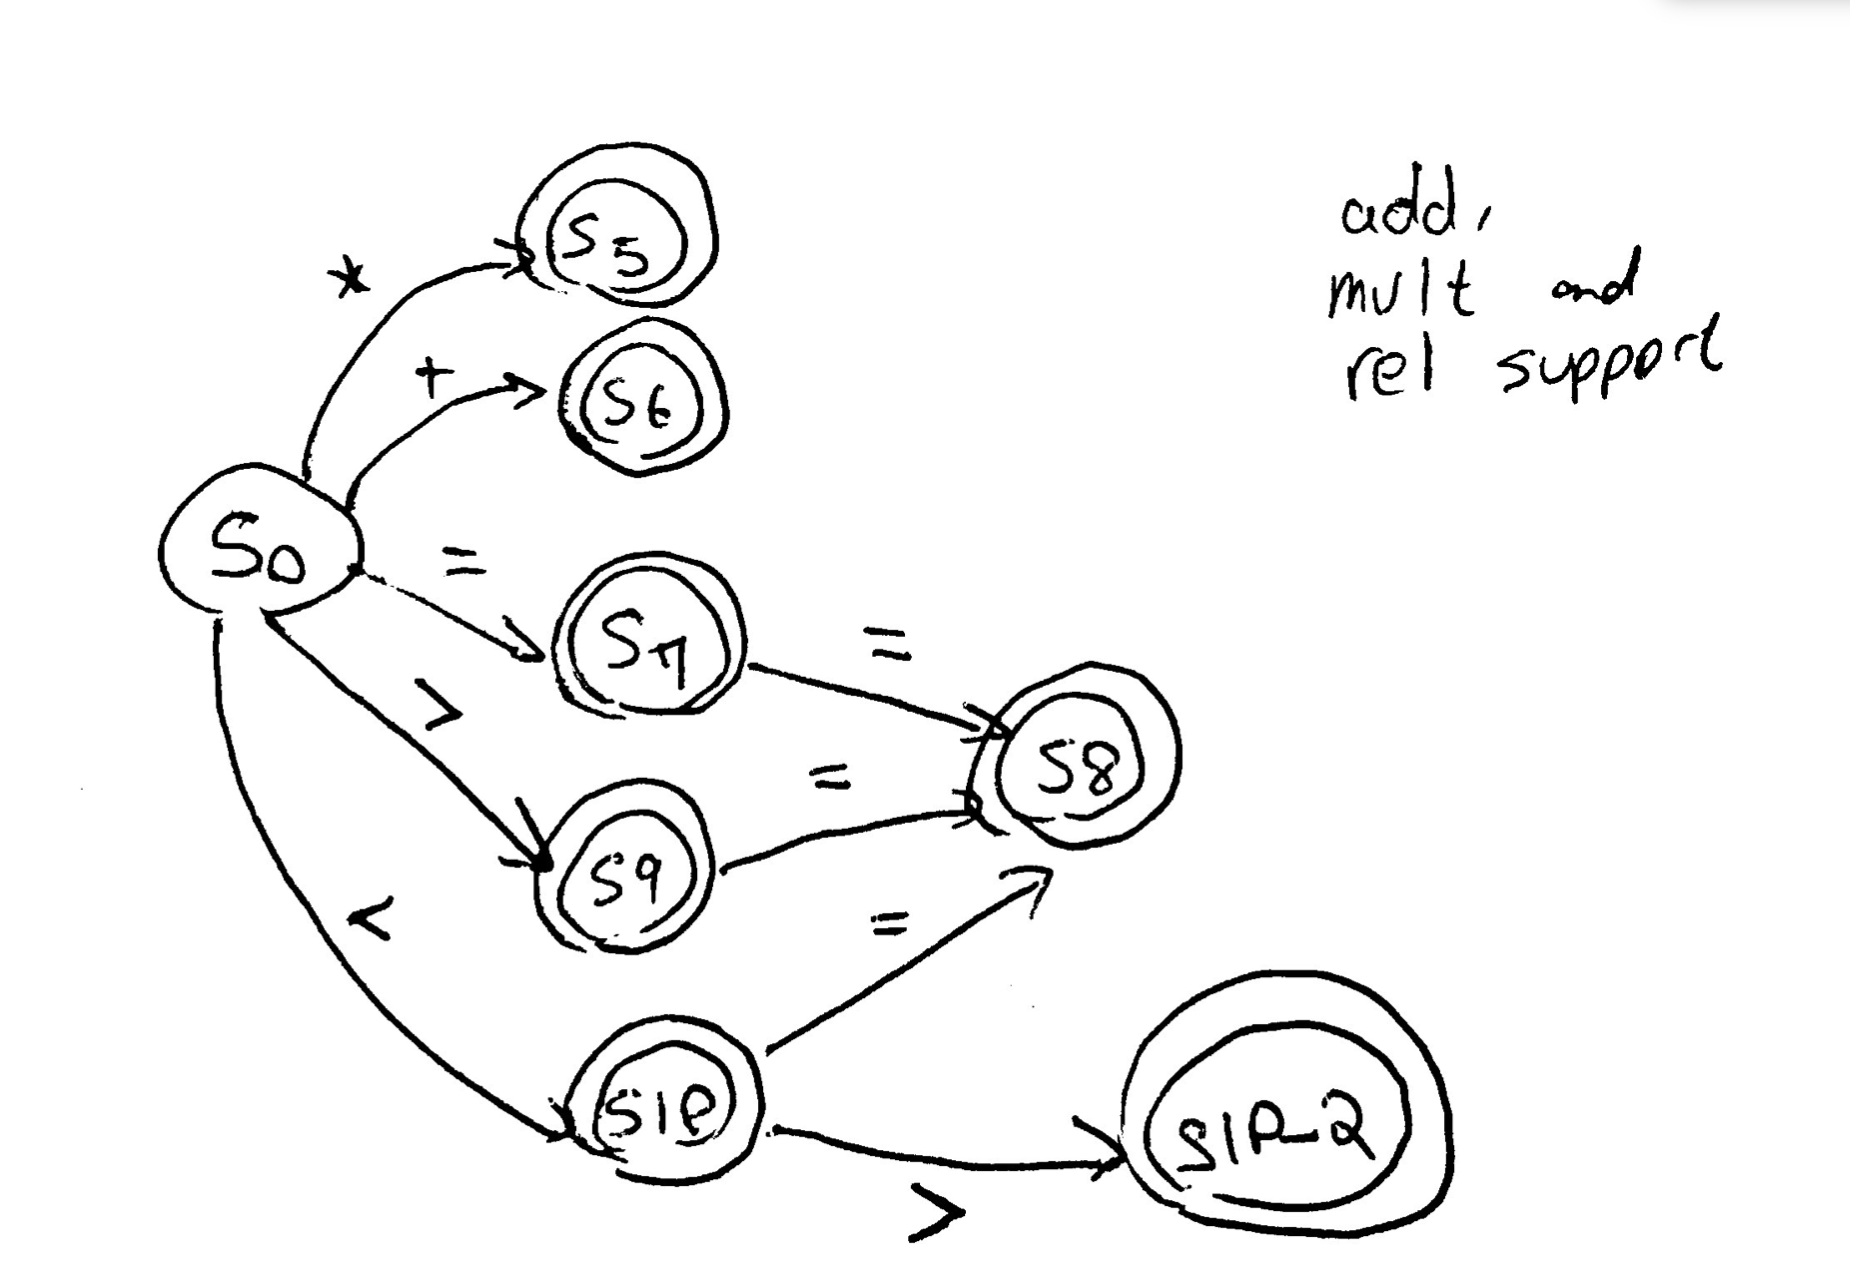
\includegraphics[width=1\textwidth]{images/operators}}
    \caption{FSA (part concerned with operators)}
\end{figure}

\begin{figure}[h]
    \centering
    \frame{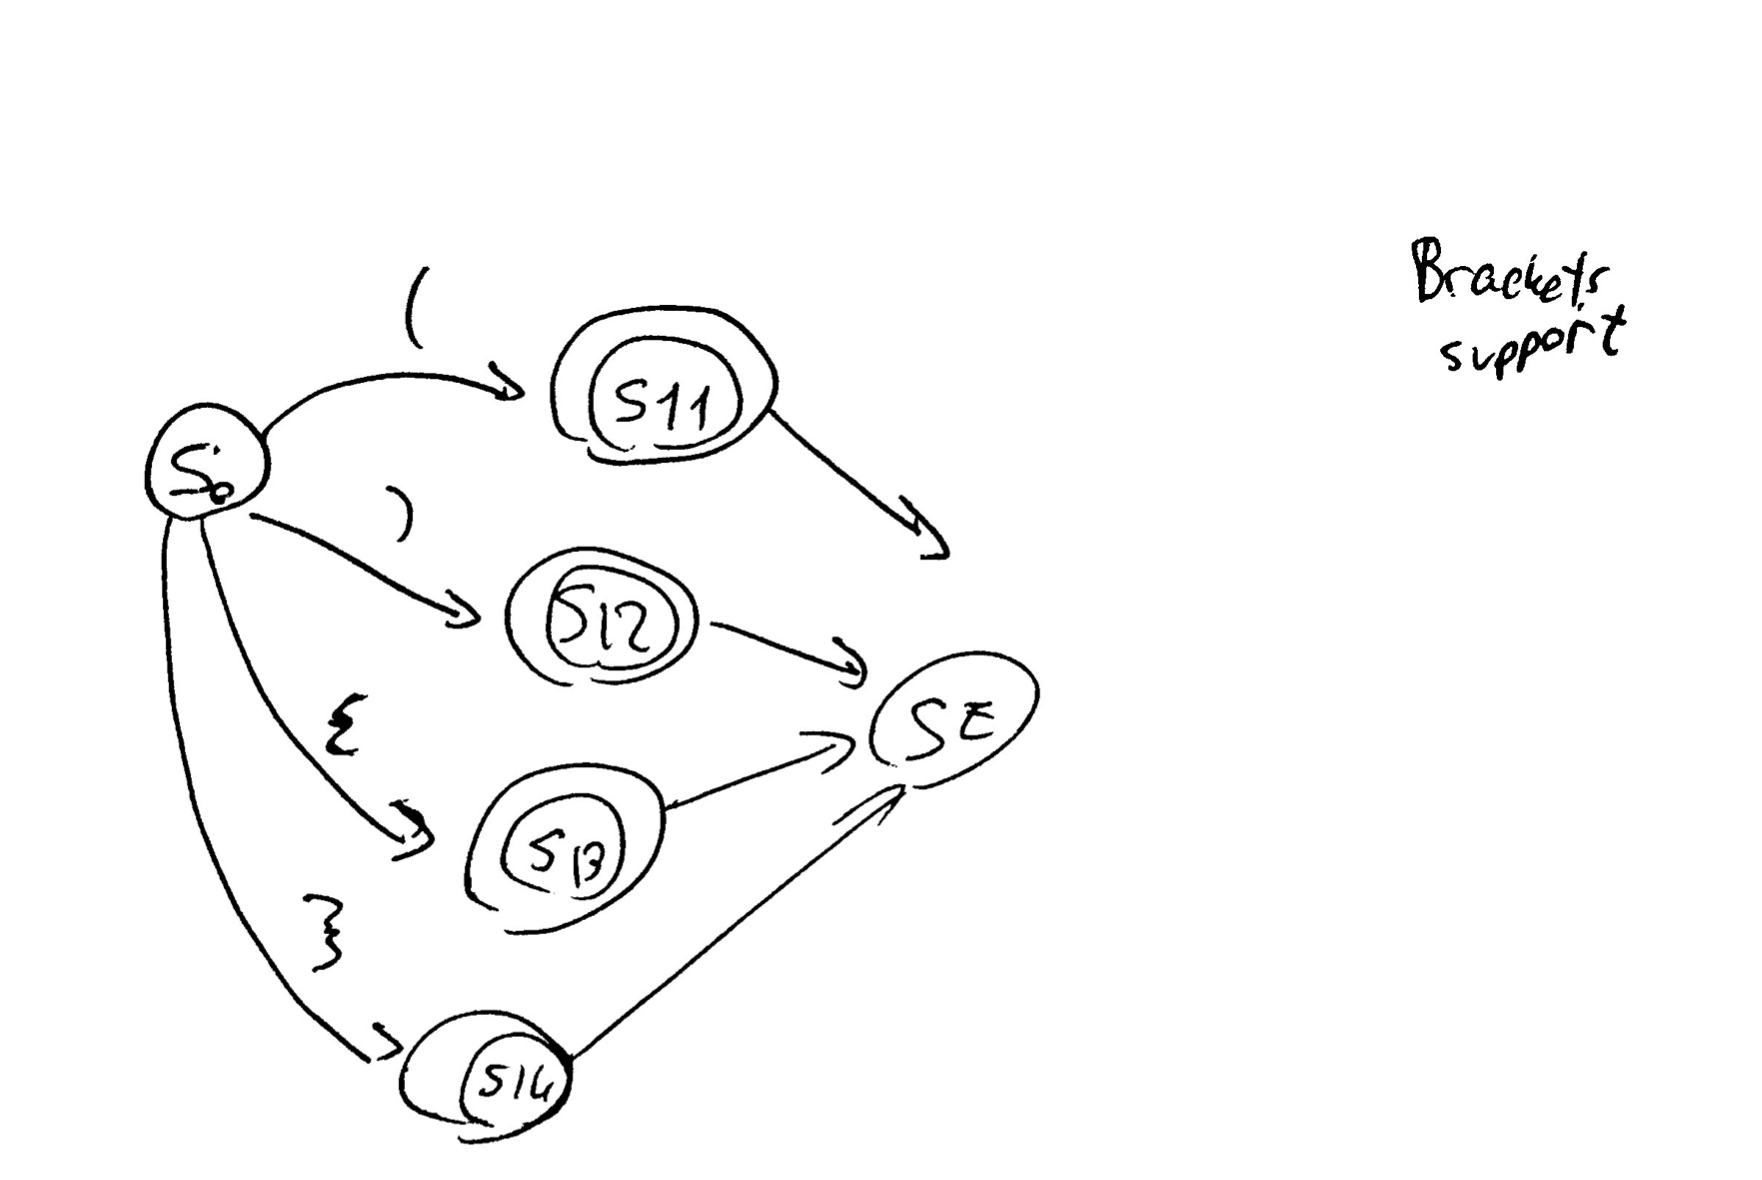
\includegraphics[width=1\textwidth]{images/brackets}}
    \caption{FSA (part concerned with brackets)}
\end{figure}


\begin{figure}[h]
    \centering
    \frame{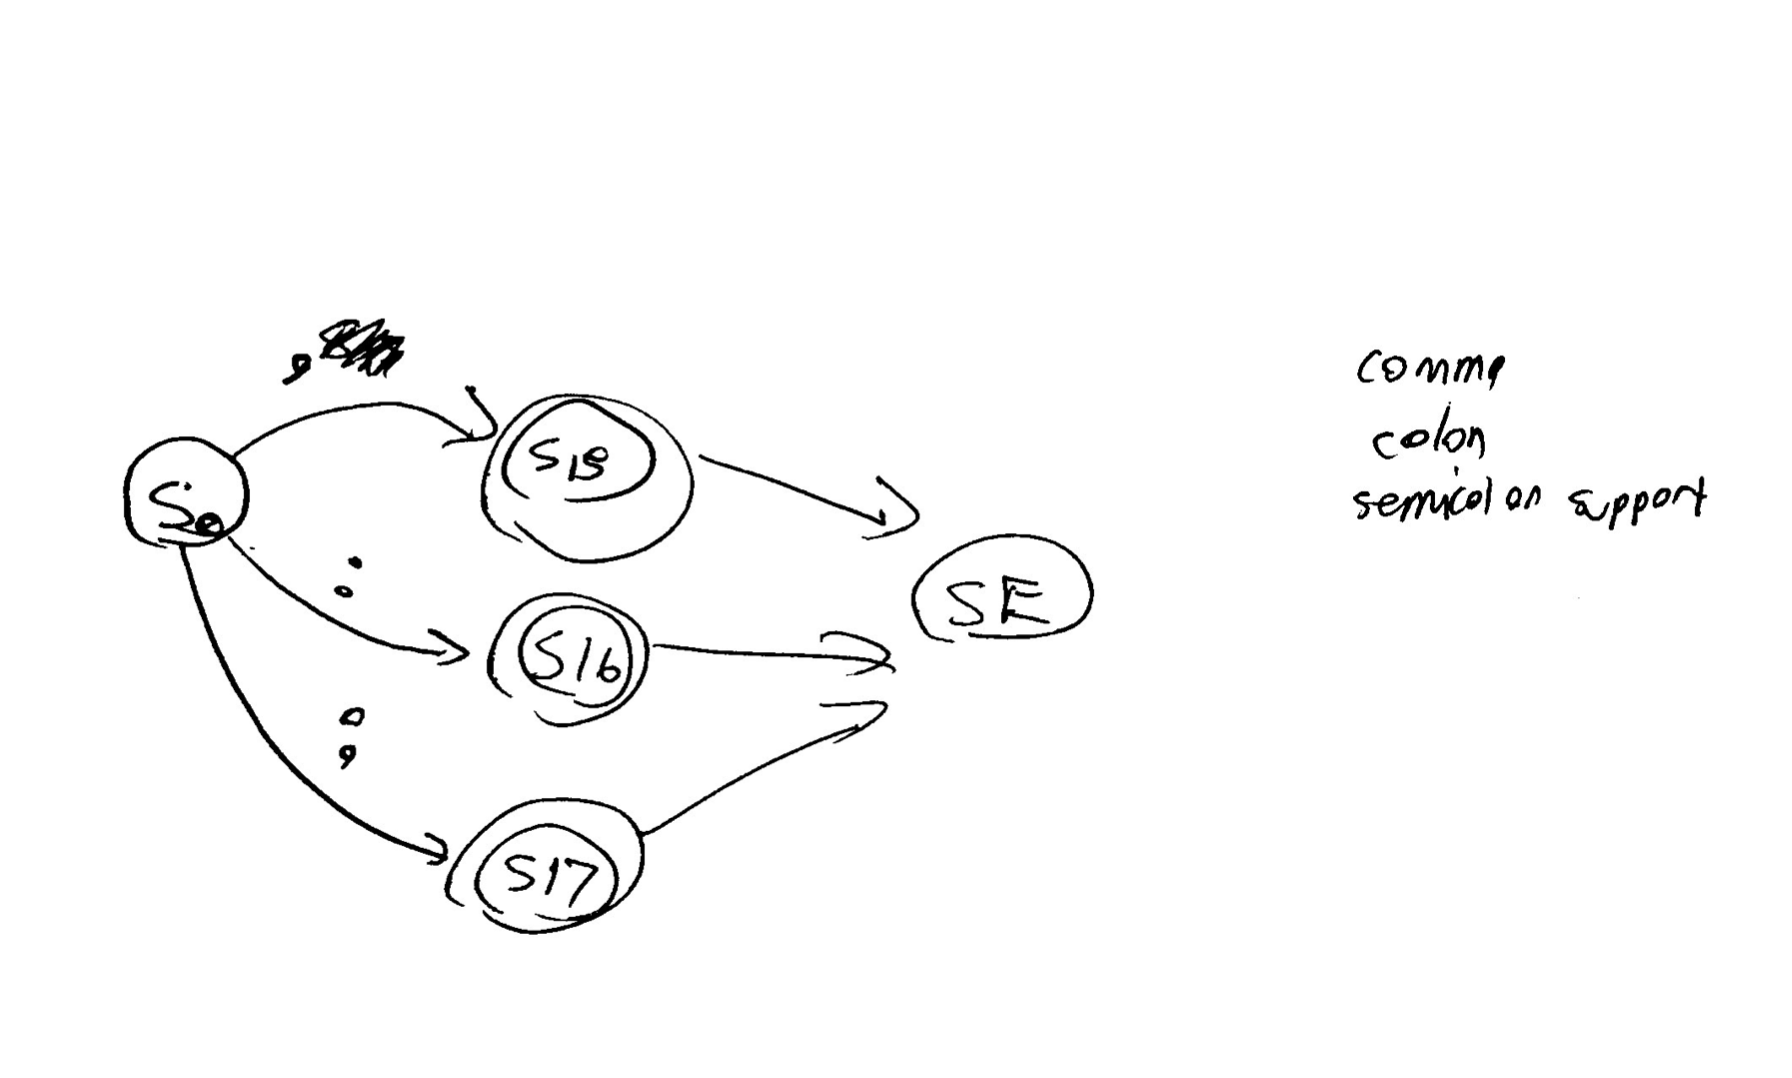
\includegraphics[width=1\textwidth]{images/colons}}
    \caption{FSA (part concerned with colons and comma)}
\end{figure}

\begin{figure}[h]
    \centering
    \frame{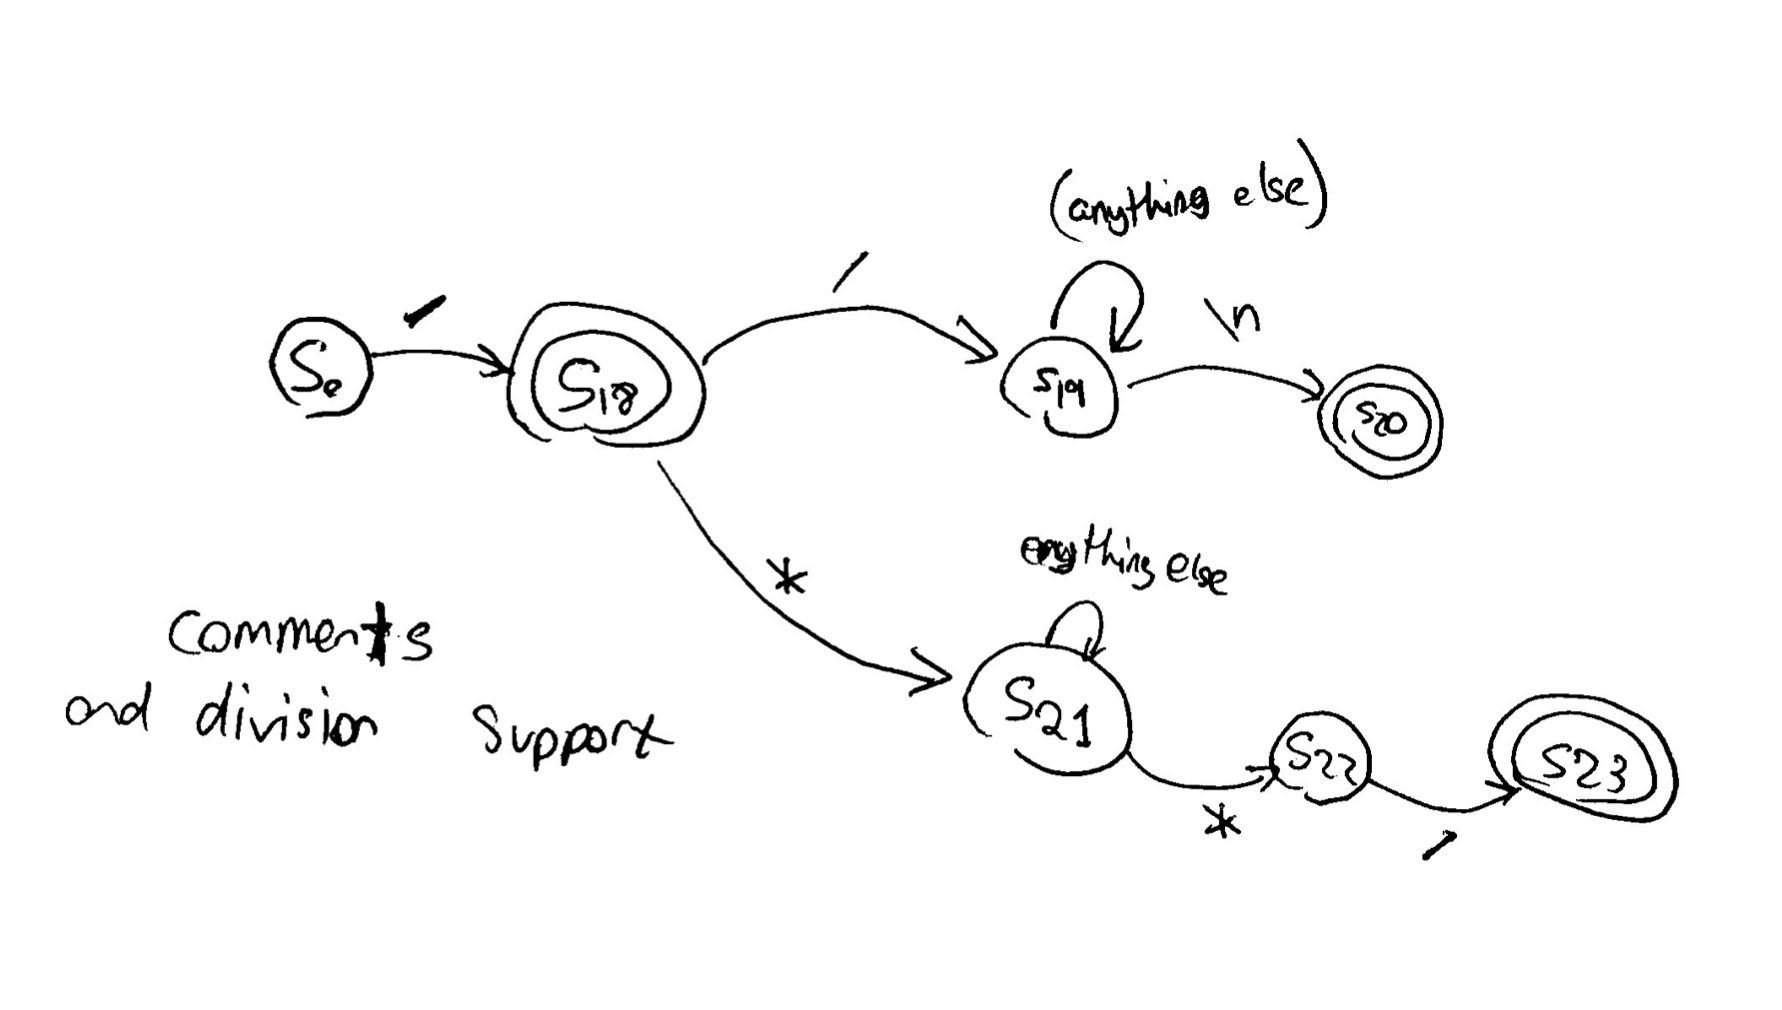
\includegraphics[width=1\textwidth]{images/comments}}
    \caption{FSA (part concerned with comments and division operator}
\end{figure}

\section{Question 2}
\subsection{How the problem was tackled}
\subsubsection{AST Nodes}
First off, the needed nodes were declared in ast.h. The nodes use inheritance to inherit features from more general nodes. These
nodes hold data about what they represent, as well as pointers to their children nodes.
\linebreak

There are three abstract nodes. ASTNode is the super class which the other two inherit from. ASTStatementNode and ASTExpressionNode
are the otehr two.
All node classes inherit from these two. The only exception is ASTProgramNode, which is the topmost node of the Abstract Syntax
Tree. This node consists of a list of statement nodes. This list is implemented
as a vector.

\subsubsection{Parser}
The parser keeps track of the current token and the next token in line. This enables its look ahead functionalitiy thus classifying 
as an LL(1) parser. It works by using the current token and the next token to check if the structure of the input program is as
valid, reporting errors if it is not.

In my implementation, functions such as parse\_if\_statement() were left out due to bad time managment from my end. However,
these would have been very similar to the ones  already implemented, as the concept is mostly the same.

\section{Question 3}
This question was not attampted.

\section{Question 4}

\end{document}
